\documentclass[a4paper,norsk, 10pt]{article}
\usepackage[utf8]{inputenc}
\usepackage{verbatim}
\usepackage{listings}
\usepackage{graphicx}
\usepackage[norsk]{babel}
\usepackage{a4wide}
\usepackage{color}
\usepackage{amsmath}
\usepackage{float}
\usepackage{amssymb}
\usepackage[dvips]{epsfig}
\usepackage[toc,page]{appendix}
\usepackage[T1]{fontenc}
\usepackage{cite} % [2,3,4] --> [2--4]
\usepackage{shadow}
\usepackage{hyperref}
\usepackage{titling}
\usepackage{marvosym }
\usepackage{subcaption}
\usepackage[noabbrev]{cleveref}
\usepackage{cite}


\setlength{\droptitle}{-10em}   % This is your set screw

\setcounter{tocdepth}{2}

\numberwithin{equation}{section}

\lstset{language=c++}
\lstset{alsolanguage=[90]Fortran}
\lstset{alsolanguage=Python}
\lstset{basicstyle=\small}
\lstset{backgroundcolor=\color{white}}
\lstset{frame=single}
\lstset{stringstyle=\ttfamily}
\lstset{keywordstyle=\color{red}\bfseries}
\lstset{commentstyle=\itshape\color{blue}}
\lstset{showspaces=false}
\lstset{showstringspaces=false}
\lstset{showtabs=false}
\lstset{breaklines}
\title{FYS2140}
\author{Kandidat nr. 15110}
\begin{document}
\maketitle

\section{Oppgave 1)}
\subsection*{a)}
Vi ønsker å se på et system med et dobbelt $\delta$-potensial. I én dimensjon er Schrödinger likningen:

$$
-\frac{\hbar^2}{2m}\frac{\partial^2 \psi(x)}{\partial x^2} + V(x)\psi(x) = E\psi(x)
$$

Vi ønsker å operere i natrulige enheter, så vi setter $\hbar = m = 1$. Som nevt skal vi se på et dobbelt $\delta$-potensial, symmetrisk om origo, og med $\delta$-funksjoner i $\pm q_0$. Dette potensialet er gitt ved:

$$
V(x) = V_0\delta(x+q_0) + V_0\delta(x-q_0)
$$

Dette gir oss en Schrödinger likning som ser slik ut:

\begin{equation}
-\frac{1}{2}\frac{\partial^2 \psi(x)}{\partial x^2} + \left[V_0\delta(x+q_0) + V_0\delta(x-q_0)\right]\psi(x) = E\psi(x)
\label{eq:deltaSchr}
\end{equation}

Vi er interessert i å se på de ubunnede tilstandene, dette betyr at $E>0$. Generelt gir dette løsningen:

$$
\psi(x) = 
\begin{cases}
Ae^{ikx} + Be^{-ikx} & x< -q_0 \\
Ce^{ikx} + De^{-ikx} & -q_0x< q_0 \\
Fe^{ikx} + Ge^{-ikx} & x>q_0 
\end{cases}
$$

Hvor $k = \sqrt{2E}$. Vi ønsker at løsningen er en bølge som kommer fra venstre. Ser vi på den nederst linjen, så er dette bølgefunksjonen på høyre siden av potensialet. $Fe^{ikx}$ tilsvarer bølgen som beveger seg på høyre, og $Ge^{-ikx}$ er bølgen som beveger seg mot venstre. Men bølgen skal komme bare fra venstre, som betyr at det som kommer seg igjennom potensialet må bevege seg mot høyre. Dette betyr at $G = 0$. Vi får da

\begin{equation}
\psi(x) = 
\begin{cases}
Ae^{ikx} + Be^{-ikx} & x< -q_0 \\
Ce^{ikx} + De^{-ikx} & -q_0x< q_0 \\
Fe^{ikx} & x>q_0 
\end{cases}
\label{eq:psi}
\end{equation}
\newpage
Vi skriver også opp de deriverte av bølgefunksjonen:


\begin{equation}
\psi'(x) = 
\begin{cases}
ikAe^{ikx} - ikBe^{-ikx} & x< -q_0 \\
ikCe^{ikx} -ikDe^{-ikx} & -q_0x< q_0 \\
ikFe^{ikx} & x>q_0 
\end{cases}
\label{eq:psiDer}
\end{equation}

Vi må nå finne de fem variablene A,B,C,D og F. Får å gjøre dette, bruker vi:

\begin{itemize}
\item Bølgefunksjonen er kontinuelig i $\pm q_0$
\item Den deriverte $\psi'$ er diskontimuelig i $\pm q_0$
\end{itemize}

Først ønsker jeg å finne hva denne diskontinuteten er. Vi ser først på $-q_0$. Vi integrerer \ref{eq:2dSch} fra $-q_0 - \epsilon$ til $-q_0 + \epsilon$:

$$
-\frac{1}{2}\int_{-q_0 - \epsilon}^{-q_0 + \epsilon}\frac{\partial^2 \psi(x)}{\partial x^2}dx + \int_{-q_0 - \epsilon}^{-q_0 + \epsilon}\left[V_0\delta(x+q_0) + V_0\delta(x-q_0)\right]\psi(x)dx = E\int_{-q_0 - \epsilon}^{-q_0 + \epsilon}\psi(x) dx
$$

Vi kan nå se på leddene. Når $\epsilon \rightarrow 0$ så vil 

$$E\int_{-q_0 - \epsilon}^{-q_0 + \epsilon}\psi(x) dx = 0$$

Første leddet blir $\frac{\partial \psi}{\partial x}$ men evaluert i grensene. Når $\epsilon \rightarrow 0$ blir dette diskontinuliteten vi er ute etter:

$$
-\int_{-q_0 - \epsilon}^{-q_0 + \epsilon}\frac{\partial^2 \psi(x)}{\partial x^2}dx = -\lim_{\epsilon \rightarrow 0}\left(\frac{\partial \psi}{\partial x}\right)\bigg|_{-q_0 - \epsilon}^{-q_0 + \epsilon} = -\Delta \left(\frac{\partial \psi}{\partial x}\right)_{-q_0}
$$

Vi ser da at

\begin{equation}
\Delta \left(\frac{\partial \psi}{\partial x}\right)_{-q_0} = 2\int_{-q_0 - \epsilon}^{-q_0 + \epsilon}\left[V_0\delta(x+q_0) + V_0\delta(x-q_0)\right]\psi(x)dx = 2V_0\psi(-q_0)
\label{eq:deltapsi-q0}
\end{equation}

Og tilsvarende

\begin{equation}
\Delta \left(\frac{\partial \psi}{\partial x}\right)_{q_0} = 2V_0\psi(q_0)
\end{equation}



Vi kan nå starte å sette opp likningssystemet:\\

\textbf{Kontinuitet i $-q_0$}: 
Vi får da at 

$$
Ae^{-ikq_0} + Be^{ikq_0} = Ce^{-ikq_0} + De^{ikq_0}
$$

Vi innfører nå variablen $\alpha = e^{-2ikq_0}$, og får:

$$
A\alpha + B =C\alpha + D
$$

\textbf{Kontinuitet i $q_0$}: 
Vi får her at:

$$
Ce^{ikq_0} + De^{-ikq_0} = Fe^{ikq_0} 
$$
$$
\Rightarrow C + D\alpha = F
$$

\newpage

\textbf{Diskontinuitet for $\psi'$ i $-q_0$}:

Vi får her at

$$
\Delta \left(\frac{\partial \psi}{\partial x}\right)_{-q_0} = (ikCe^{-ikq_0} -ikDe^{ikq_0} ) - (ikAe^{-ikq_0} - ikBe^{ikq_0}) = 2V_0\psi(-q_0) 
$$
$$
= 2V_0(Ae^{-ikq_0} + Be^{ikq_0})
$$
$$
\Rightarrow ik(C\alpha - D -A\alpha + B) = 2V_0(A\alpha + B)
$$

Vi innfører så en ny variablel $\omega = \frac{2V_0}{ik}$ og får:

$$
\Rightarrow C\alpha - D -A\alpha + B = \omega(A\alpha + B)
$$

\textbf{Diskontinuitet for $\psi'$ i $q_0$}:
Vi får her:

$$
\Delta \left(\frac{\partial \psi}{\partial x}\right)_{q_0} = ikFe^{ikq_0} - (ikCe^{ikq_0} -ikDe^{-ikq_0}) = 2V_0\psi(q_0)
$$
$$
= 2V_0Fe^{ikq_0}
$$
$$
\Rightarrow F - C + D\alpha = \omega F 
$$\\


Vi sitter da med de fire likningene for de fem ukjente:

\begin{enumerate}
\item $A\alpha + B = C\alpha + D$
\item $C + D\alpha = F$
\item $C\alpha - D -A\alpha + B = \omega(A\alpha + B)$
\item $F - C + D\alpha = \omega F $
\end{enumerate}

Hvor $\alpha = e^{-2ikq_0}$ og $\omega = \frac{2V_0}{ik}$.\\

Det er fult mulig å løse dette analytisk, men etter mange forsøk og mange blindveier så ble jeg inspirert av noen andre til bare å løse dette ved hjep av \textit{sympy}, en symbolsk løser for python.Koden finnes her\ref{lst:solver}. Den ga dette resultatet:

$$
F = \frac{4A\alpha^2}{\alpha^2\omega^2 - 4\alpha^2\omega + 4\alpha^2 - \omega^2}
$$
$$
B = \frac{A\alpha\omega(2+\omega +2\alpha^2 - \alpha^2\omega)}{\alpha^2\omega^2 - 4\alpha^2\omega + 4\alpha^2 - \omega^2}
$$
$$
C = \frac{-2A\alpha^2(\omega - 2)}{\alpha^2\omega^2 - 4\alpha^2\omega + 4\alpha^2 - \omega^2}
$$
$$
D = \frac{2A\alpha\omega}{\alpha^2\omega^2 - 4\alpha^2\omega + 4\alpha^2 - \omega^2}
$$

Setter vi inn for $\alpha$ og $\omega$ og rydder litt, finner vi:

$$
F = \frac{4Ae^{-4ikq_0}}{-\frac{4V_0^2}{k^2}e^{-4ikq_0} + \frac{8iV_0}{k}e^{-4ikq_0} + 4e^{-4ikq_0} + \frac{4V_0^2}{k^2}}
$$
$$
= \frac{4Ae^{-4ikq_0}}{2iV_0k + k^2 +V_0^2e^{4ikq_0} - V_0^2}\frac{1}{\frac{4e^{-4ikq_0}}{k^2}}
$$

\begin{equation}
= \frac{Ak^2}{2iV_0k + k^2 +V_0^2e^{4ikq_0} - V_0^2}
\label{eq:F}
\end{equation}

Og for de resterende:

\begin{equation}
B = -\frac{AV_0\left(V_0e^{2ikq_0} - V_0e^{-2ikq_0} + ike^{2ikq_0} + ike^{-2ikq_0}\right)}{2iV_0k + k^2 +V_0^2e^{4ikq_0} - V_0^2}
\label{eq:B}
\end{equation}

\begin{equation}
C = \frac{Ak(iV_0 + k)}{2iV_0k + k^2 +V_0^2e^{4ikq_0} - V_0^2}
\label{eq:C}
\end{equation}

\begin{equation}
D = \frac{-AikV_0e^{2ikq_0}}{2iV_0k + k^2 +V_0^2e^{4ikq_0} - V_0^2}
\label{eq:D}
\end{equation}

Setter vi nå disse inn i \ref{eq:psi} får vi spredningstilstandene:

\begin{equation}
\psi(x) =
\begin{cases}
Ae^{ikx} -\frac{AV_0\left(V_0e^{2ikq_0} - V_0e^{-2ikq_0} + ike^{2ikq_0} + ike^{-2ikq_0}\right)}{2iV_0k + k^2 +V_0^2e^{4ikq_0} - V_0^2}e^{-ikx} & x< -q_0 \\
\frac{Ak(iV_0 + k)e^{ikx} -AikV_0e^{2ikq_0}e^{-ikx}}{2iV_0k + k^2 +V_0^2e^{4ikq_0} - V_0^2} & -q_0x< q_0 \\
\frac{Ak^2}{2iV_0k + k^2 +V_0^2e^{4ikq_0} - V_0^2}e^{ikx} & x>q_0 
\end{cases}
\end{equation}

Jeg er ganske sikker på at det finnes måter å forenkle dette på. Siden \textit{sympy} ikke er like flink som mennesker til å rydde opp i uttrykk, så blir det ganske rotete. Men det skal være riktig.


\subsection*{b)}

Vi kan nå begynne å se på hvor mye som blir reflektert, og hvor mye som blir transmittert. Vi skal først se på hvor mye som blir reflektert av $\delta$-funksjonen i $x = -q_0$. Vi er interessert i hva som er sjansen for at bølgen blir reflektert. Dette kan vi gjøre med refleksjonskoeffisienten:

\begin{equation}
R = \frac{|B|^2}{|A|^2}
\label{eq:refleks}
\end{equation}

Vi kan regne dette ut:

$$
R = \frac{|B|^2}{|A|^2} = \bigg|\frac{V_0\left(V_0e^{2ikq_0} - V_0e^{-2ikq_0} + ike^{2ikq_0} + ike^{-2ikq_0}\right)}{2iV_0k + k^2 +V_0^2e^{4ikq_0} - V_0^2}\bigg|^2
$$

Bruker vi sympy, wolframalpha eller liknende til å regne ut dette finner vi at 

$$
R = \frac{V_0\left(k\cos(2kq_0) + V_0\sin(2kq_0)\right)^2}{4kV_0^3\sin(4kq_0) + 2V_0^2\cos(4kq_0)(k^2 - V_0^2)+k^4 +2k^2V_0^2 + 2V_0^4}
$$

Vi kan sette inn $k = \sqrt{2E}$ for å finne den endelige sannsyligheten som en funksjon av $E$, $q_0$ og $V_0$:

$$
R(E,q_0,V_0) = \frac{V_0\left(\sqrt{2E}\cos(2\sqrt{E}q_0) + V_0\sin(2\sqrt{2E} q_0)\right)^2}{4\sqrt{2E}V_0^3\sin(4\sqrt{2E} q_0) + 2V_0^2\cos(4\sqrt{2E} q_0)(2E - V_0^2)+4E^2 +4EV_0^2 + 2V_0^4}
$$

Vi ønsker så å gjøre det tilsvarende for transmisjonen gjennom det høyre potensialet. Dette måler sannsynligheten for at bølgen har gått igjennom hele potensialet for forsvinner mot høyre. Dette kan regnes ut som følger:

\begin{equation}
T = \frac{|F|^2}{|A|^2}
\label{eq:transmit}
\end{equation}

Jeg brukte akkurat samme metode som jeg brukte for refleksjonsmetoden (symbolske løsere):

$$
T = \bigg|\frac{k^2}{2iV_0k + k^2 +V_0^2e^{4ikq_0} - V_0^2}\bigg| 
$$
$$
= \frac{k^4}{(2iV_0k + k^2 +V_0^2e^{4ikq_0} - V_0^2)(-2iV_0k + k^2 +V_0^2e^{-4ikq_0} - V_0^2)}
$$
$$
 = \frac{k^4}{4kV_0^3\sin(4kq_0) + 2V_0^2\cos(4kq_0)(k^2 - V_0^2)+k^4 +2k^2V_0^2 + 2V_0^4}
$$

Setter vi så inn $k = \sqrt{2E}$ finner vi transmisjonssannsynligheten som

\begin{equation}
T(E,q_0,V_0) = \frac{4E^2}{4\sqrt{2E}V_0^3\sin(4\sqrt{2E} q_0) + 2V_0^2\cos(4\sqrt{2E} q_0)(2E - V_0^2)+4E^2 +4EV_0^2 + 2V_0^4}
\end{equation} 

Som en test på at det ikke er feil,så kan vi observere at enten må bølgen reflekteres eller så må den komme ut på andre siden. Dette betyr at 

$$
T + R \overset{!}{=} 1
$$


Vi kan sjekke dette:

$$
T + R = \frac{V_0\left(\sqrt{2E}\cos(2\sqrt{E}q_0) + V_0\sin(2\sqrt{2E} q_0)\right)^2 + k^4}{4\sqrt{2E}V_0^3\sin(4\sqrt{2E} q_0) + 2V_0^2\cos(4\sqrt{2E} q_0)(2E - V_0^2)+4E^2 +4EV_0^2 + 2V_0^4}
$$

Sjekker man dette på de symbolske løserne finner vi utrolig nok at:

$$
V_0\left(\sqrt{2E}\cos(2\sqrt{E}q_0) + V_0\sin(2\sqrt{2E} q_0)\right)^2 + k^4
$$
$$
= 4\sqrt{2E}V_0^3\sin(4\sqrt{2E} q_0) + 2V_0^2\cos(4\sqrt{2E} q_0)(2E - V_0^2)+4E^2 +4EV_0^2 + 2V_0^4
$$

Hvilke betyr at

$$
T + R = \frac{4\sqrt{2E}V_0^3\sin(4\sqrt{2E} q_0) + 2V_0^2\cos(4\sqrt{2E} q_0)(2E - V_0^2)+4E^2 +4EV_0^2 + 2V_0^4}{4\sqrt{2E}V_0^3\sin(4\sqrt{2E} q_0) + 2V_0^2\cos(4\sqrt{2E} q_0)(2E - V_0^2)+4E^2 +4EV_0^2 + 2V_0^4} = \underline{\underline{1}}
$$

Vi har derfor vist at løsningen består en av de viktigste testene for refleksjons- og transmisjonkoeffisientene!

\textit{Merknad: Mye av det jeg har gjort i denne deloppgaven skal være mulig å gjøre analytisk. Men siden jeg løste forrige deloppgave med sympy så fikk jeg svarene på slik en måte at det ble mer eller mindre å løse ting analytisk. Personer som løste 1a analytisk vil nok kunne løse 1b på samme måte. Jeg vet at noen har gjort dette. Men jeg er likevel sikker på at det jeg har skrevet er helt korrekt, bare på en litt mer komplisert form.}

\newpage
\subsection*{c)}

Merk at jeg var dum og brukte $k = \sqrt{2E}$, for nå som vi skal se på den transmitterte fluksen til et vanlig $\delta$-potensial, brukes allerede $k = \frac{\sqrt{2E}}{V_0}$. Jeg velger derfor her heller å skrive $\kappa = \frac{\sqrt{2E}}{V_0}$. Den transmitterte fluken til ett $\delta$-potensial er derfor gitt som

$$
T = \frac{\kappa^2}{1 + \kappa^2}
$$

Vi kan plotte denne transmitterings fluksen mot den for det dobble $\delta$-potensialet:

\begin{figure}[H]
\centering
\begin{subfigure}{0.3\textwidth}
\centering
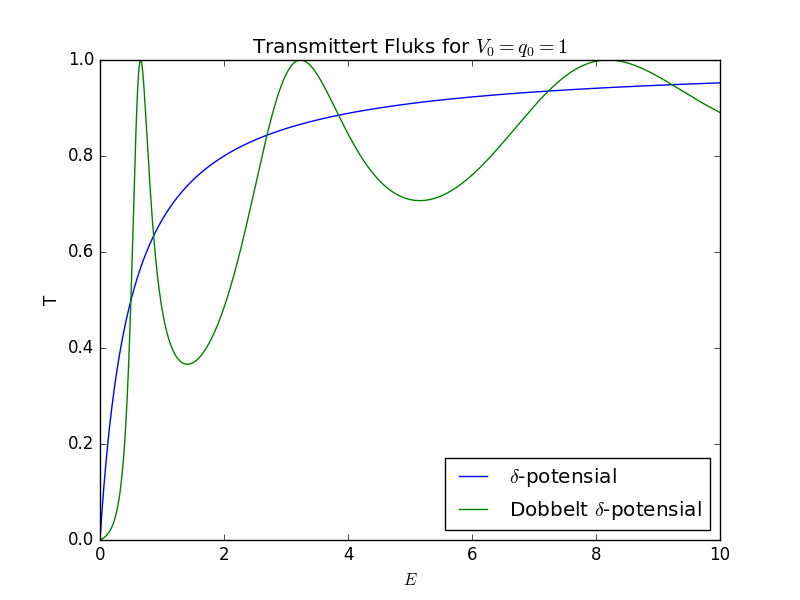
\includegraphics[width = \textwidth]{TE.png}
\caption{Den transmitterte fluksen som en funksjon av E}
\label{fig:TE}
\end{subfigure}
~
\begin{subfigure}{0.3\textwidth}
\centering
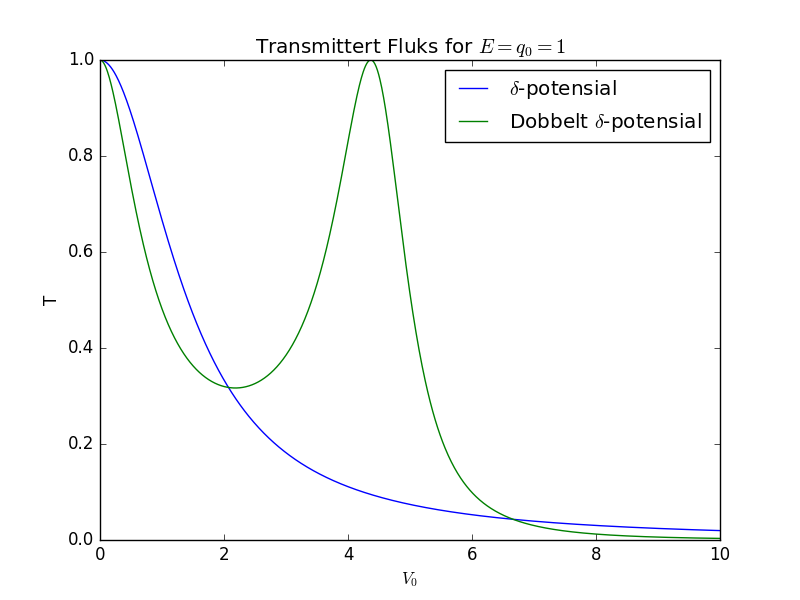
\includegraphics[width = \textwidth]{TV.png}
\caption{Den transmitterte fluksen som en funksjon av $V_0$}
\end{subfigure}
\end{figure}


Vi kan se at det er enkelte steder hvor det transmitteres mer ved et dobbelt potensial enn ved et enkelt. Vi ønsker å se litt nærmere på når dette skjer. La oss ta en liten titt på \ref{fig:TE}. Vi kan se at $T = 1$ for energiene $E \approx 0.67$, $E \approx 3.25$ og $E \approx 8.22$. La oss plotte $|\psi|^2$ for området i mellom $\delta$-funksjonene:

\begin{figure}[H]
\centering
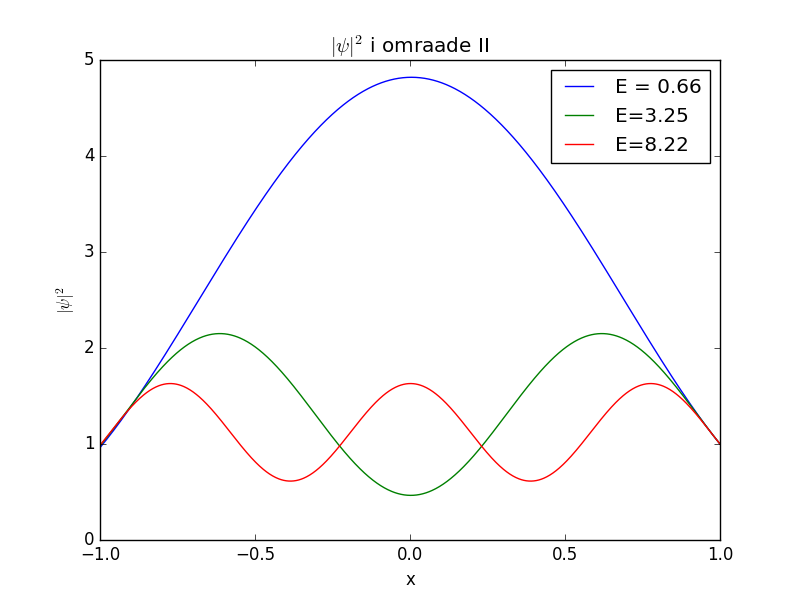
\includegraphics[scale=0.5]{psi2omr2.png}
\caption{Vi ser at for disse energiene er bølgene i område $II$ stående bølger med $n+1$ bølgetopper.}
\end{figure}

Det ser ut som om når den transmitterte fluksen nærmer seg 1, så er det stående bølger i område $II$. Det kan se ut som ved enkelte verdier av $q_0$,$E$ og $V_0$ oppstår disse stående bølgene. Men får da konstruktiv resonnans. Dette kan virke som denne resonnasen forusaker en høyere transmisjonsfluks. Dette er noe som ikke oppstår ved en enkel $\delta$-funksjon, og vi får derfor en høyere transmittert fluks igjennom det doble $\delta$-potensialet.\\


Vi kan sjekke hvilke verdier for $q_0$ som gir størst transmisjon for $E = V_0 = 1$. Her blir

$$
T(q_0) = \frac{4}{4\sqrt{2}\sin(4\sqrt{2} q_0) + 2\cos(4\sqrt{2} q_0)(2 - 1)+4 +4 + 2}
$$

Den største mulighe transmitterte fluksen er 1, hvilke betyr at:

$$
4\sqrt{2}\sin(4\sqrt{2} q_0) + 2\cos(4\sqrt{2} q_0)+10 = 4
$$

Dette gir oss at:

$$
q_0 = \frac{n\pi - \arctan(\sqrt{2}}{2\sqrt{2}}, \qquad n= 0,1,2,...
$$

Dette er altså den sperasjonen av $\delta$-funksjonene som gir høyest transmisjon.


\section{Oppgave 2)}

\subsection*{a)}

Den tidsuavhengige Schrödinger likningen er gitt som 

\begin{equation}
\hat{H}\psi = E\psi
\label{eq:TUSL}
\end{equation}

Hvor $E$ er energien til systemet, mens $\hat{H}$ er den hamiltonske operatoren. Denne er gitt som

$$
\hat{H} = -\frac{\hbar^2}{2m}\nabla^2  + V(x,y)
$$

I 2 dimensjoner er:

$$
\nabla^2 = \frac{\partial^2}{\partial x^2} + \frac{\partial^2}{\partial y^2}
$$

Vi skal se på tilfelle hvor potensialet er det for en 2 dimensjonal harmonisk osillator:

$$
V(x,y) = \frac{1}{2}m\omega^2(x^2 + y^2)
$$

Dette gir oss Schrödinger likningen for dette systemet:

\begin{equation}
-\frac{\hbar^2}{2m}\left(\frac{\partial^2 \psi}{\partial x^2} + \frac{\partial^2 \psi}{\partial y^2}\right) + \frac{1}{2}m\omega^2(x^2 + y^2)\psi = E\psi
\label{eq:2dSch}
\end{equation}

\subsection*{b)}

Vi kan se at det er mulig å separere differensiallikningen inn i to likninger bare avhengig av enten $x$ eller $y$. Funksjonen $\psi$ kan derfor skrives som et produkt av løsningene på disse to likningene. Disse to løsningene kaller vi $X = X(x)$ og $Y = Y(y)$. $\psi$ kan derfor skrives som

$$
\psi(x,y) = X(x)Y(y)
$$

Vi kan sette dette inn i \ref{eq:2dSch}

$$
-\frac{\hbar^2}{2m}\left(\frac{\partial^2 XY}{\partial x^2} + \frac{\partial^2 XY}{\partial y^2}\right) + \frac{1}{2}m\omega^2(x^2 + y^2)XY = EXY
$$


Siden $X$ er uavhenging av $y$ og $Y$ av $x$, så kan vi stokke litt om på derivasjonene:

$$
-\frac{\hbar^2}{2m}\left(Y\frac{\partial^2 X}{\partial x^2} + X\frac{\partial^2 Y}{\partial y^2}\right) + \frac{1}{2}m\omega^2(x^2 + y^2)XY = EXY
$$

Vi deler så hele likningen på $XY$:

$$
-\frac{\hbar^2}{2m}\left(\frac{1}{X}\frac{\partial^2 X}{\partial x^2} + \frac{1}{Y}\frac{\partial^2 Y}{\partial y^2}\right) + \frac{1}{2}m\omega^2(x^2 + y^2) = E
$$

Vi stokke om og samle de delene som er avhengig av samme variabel:

\begin{equation}
\underbrace{-\frac{\hbar^2}{2m}\frac{1}{X}\frac{\partial^2 X}{\partial x^2} + \frac{1}{2}m\omega^2x^2}_{E_x} + \underbrace{-\frac{\hbar^2}{2m}\frac{1}{Y}\frac{\partial^2 Y}{\partial y^2} + \frac{1}{2}m\omega^2y^2}_{E_y} = E
\label{eq:ExEy}
\end{equation}


Jeg har her kalt de to leddene $E_x$ og $E_y$, og dette er ikke uten grunn. Om vi nå skriver disse likningene over hver for seg:

$$
-\frac{\hbar^2}{2m}\frac{1}{X}\frac{\partial^2 X}{\partial x^2} + \frac{1}{2}m\omega^2x^2 = E_x
$$
$$
-\frac{\hbar^2}{2m}\frac{1}{Y}\frac{\partial^2 Y}{\partial y^2} + \frac{1}{2}m\omega^2y^2 = E_y
$$

Vi ganger så likningene med forholdsvis $X$ og $Y$:

$$
-\frac{\hbar^2}{2m}\frac{\partial^2 X(x)}{\partial x^2} + \frac{1}{2}m\omega^2x^2X(x) = E_xX(x)
$$
$$
-\frac{\hbar^2}{2m}\frac{\partial^2 Y(y)}{\partial y^2} + \frac{1}{2}m\omega^2y^2Y(y) = E_yY(y)
$$

Det vi nå kan se at de to differensiallikningene vi har fått er 2 likninger som tilsvarer Schrödinger likninger for harmoniske osillatorer i $x$- og $y$-retning. Dette betyr at den 2 dimensjonale harmoniske osillatoren bare består av 2 lineært uavhengige harmoniske osillatorer, én i $x$-retning og én i $y$-retning! $E_x$ og $E_y$ forholdsvis energien til den harmoniske osillatoren i $x$- og $y$-retningen. Fra \ref{eq:ExEy} ser vi at

$$
E = E_x +E_y
$$

Siden vi kan skrive $\psi = X_i(x)Y_j(y)$, hvor $i$ og $j$ er kvantetall assosiert med de harmoniske osillatorene i de 2 retningene, og $E = E_x + E_y$, så betyr det at det er flere konfigurasjoner av disse kvantetallene kan gi samme energi $E$. Dette betyr at dette systemet er \textit{degenerert}.

\newpage

\section{Oppgave 3)}

\subsection*{a)}
Vi har en observabel beskrevet av den hermitiske matrisen

\begin{equation}
D =
\begin{pmatrix}
0 &1\\
1 &2
\end{pmatrix}
\end{equation}

Dette er en operator som kan brukes på tilstandene til et system som så gir de faktiske målingene. Tilstandene til systemet er gitt som egenvektorene til $D$, mens målingene er gitt som egenverdiene til $D$. Vi bruker Dirac-notasjon, som gjør at dette skrives  som \textit{keter}:

$$
\hat{D}|d_{\pm}\rangle = d_{\pm}|d_{\pm}\rangle
$$

Her er $|d_{\pm}\rangle$ de to tilstandsegenvektorene, mens $d_{\pm}$ er målingsegenverdiene. Dette kan være litt forvirrende notasjon, men egenvektorene er alltid inni en \textit{ket}, $|$ $\rangle$(eller senere inni en \textit{bra} $\langle$ $|$, mens egenverdier står som  'frittstående' tall\\

Vi starter med å finne egenverdien. Dette gjøres på standardmetoden:

$$
\begin{vmatrix}
0 - d & 1\\
1 & 2-d
\end{vmatrix}
= d^2 - 2d - 1 = 0
$$

Svaret på dette karakteristiske polynomet er 

$$
d_{\pm} = \frac{2 \pm \sqrt{4 + 4}}{2} = 1\pm \sqrt{2}
$$

De mulige målingene for observablen $D$ er derfor $d_{\pm} = 1 \pm \sqrt{2}$. Vi kan bruke dette til å finne tilstandene, i form av egenvektorene til disse to egenverdiene. Egenvektorene til egenverdiene er definert som nullrommet til $D - d_{\pm}I$. Vi starter med egenverdien til $d_+ = 1 + \sqrt{2}$

$$
Null
\begin{pmatrix}
0 -1 - \sqrt{2} & 1\\
1 & 2 -1 - \sqrt{2}
\end{pmatrix}
= 
\begin{pmatrix}
-1 + \sqrt{2}\\
1
\end{pmatrix}
$$

Normaliserer vi dette finner vi den første egenvektoren:

\begin{equation}
|d_+\rangle = \frac{1}{\sqrt{4-2\sqrt{2}}}
\begin{pmatrix}
-1 + \sqrt{2}\\
1
\end{pmatrix}
\label{eq:d+}
\end{equation}


Vi regner så ut egenvektoren til $d_- = 1-\sqrt{2}$:
$$
Null
\begin{pmatrix}
0 -1 + \sqrt{2} & 1\\
1 & 2 -1 + \sqrt{2}
\end{pmatrix}
= 
\begin{pmatrix}
-1 - \sqrt{2}\\
1
\end{pmatrix}
$$

Og så normaliserer den og finner den andre egenvektoren:

\begin{equation}
|d_-\rangle = \frac{1}{\sqrt{4+2\sqrt{2}}}
\begin{pmatrix}
-1 - \sqrt{2}\\
1
\end{pmatrix}
\label{eq:d-}
\end{equation}

Vi har da funnet de mulige målingene $d_{\pm} = 1 \pm \sqrt{2}$, med de tilsvarende tilstandene til systemet $|d_+\rangle$ og $|d_-\rangle$.

\subsection*{b)}

For en observabel $D$ er gjennomsnittverdien/forventningsverdien gitt som

$$
\langle D\rangle = \langle\Psi | D | \Psi \rangle
$$

Vi vet hva $D$ er, men vi har enda ikke funnet $\Psi(t)$. For å finne denne må vi se på de to Hamiltonoperatorene:

$$
H_0 = 
\begin{pmatrix}
0 & -4\\
-4 & 6
\end{pmatrix}
, \qquad
H_1 = 
\begin{pmatrix}
1 & 0\\
0 & 3
\end{pmatrix}
$$

Vi ønsker å finne tilstandene og energiene til disse to systemene. Akkurat som i forrige deloppgave er dette gitt ved egenvektorene og egenverdiene til de to operatorene. \\

\textbf{$\underline{H_0}$}: Vi skal første finne energiene til $H_0$. Dette er egenvektorene $E_{00}$ og $E_{01}$:

$$
\begin{vmatrix}
-E_0 & -4\\
-4 & 6-E_0
\end{vmatrix}
= E_0^2 -6E_0 - 16 = 0
$$
Dette gir egenverdiene:

$$
E_0 = \frac{6 \pm \sqrt{36 + 4\cdot 16}}{2} = 3\pm 5
$$

Så vi får $E_{00} = -2$ og $E_{01} = 8$. Jeg viste hvordan man regner ut egenvektorer og normaliserer dem i forrige deloppgave, så her gir jeg bare egenvektorene som tilhører egenverdiene. For $E_{00}$

\begin{equation}
|h_{00}\rangle = \frac{1}{\sqrt{5}}
\begin{pmatrix}
2\\ 1
\end{pmatrix}
\label{eq:h00}
\end{equation}

Og for $E_{01}$:

\begin{equation}
|h_{01}\rangle = \frac{1}{\sqrt{5}}
\begin{pmatrix}
-1\\ 2
\end{pmatrix}
\label{eq:h01}
\end{equation}

\textbf{$\underline{H_1}$}: Vi kan så finne tilstandene og energiene til $H_1$. Energiene er egenvektorene, som vi som vanlig finner ved:

$$
\begin{vmatrix}
1-E_1 & 0\\
0 & 3-E_1
\end{vmatrix}
= (1-E_1)(3-E_1) = 0
$$

Dette energiene $E_{10} = 1$ og $E_{11} = 3$, med de tilsvarende egenvektorene:

\begin{equation}
|h_{10}\rangle = 
\begin{pmatrix}
1\\0
\end{pmatrix}
\label{eq:h10}
\end{equation}

og 

\begin{equation}
|h_{11}\rangle = 
\begin{pmatrix}
0\\1
\end{pmatrix}
\label{eq:h11}
\end{equation}\\

Vi er nå i stand til å finne $\Psi$. I følge oppgaven starter systemet i grunntilstanden. Dette vil si tilstanden som tilsvarer den laveste energien til $H_0$, så:

$$
\Psi_0(0) = |h_{00}\rangle = \frac{1}{\sqrt{5}}
\begin{pmatrix}
2\\1
\end{pmatrix}
$$

Denne er for øyeblikket tidsuavhengig. Men ved tiden $t_D$ er vi i regime til $H_1$, det betyr at vi må beskrive $\Psi_0(0)$ i $H_1$-system, m.a.o. som en lineærkombinasjon av egenvektorene til $H_1$, $|h_{10}\rangle$ og $|h_{11}\rangle$. Siden disse er det samme som basisvektorene til $\mathbb{R}^2$ ($\hat{e}_0$ og $\hat{e}_1$), så er dette en enkel oppgave:

$$
\Psi_0(t) = \frac{1}{\sqrt{5}}(2|h_{10}\rangle + |h_{11}\rangle)
$$

Vi kan så legge til en tidsavhengighet ved hjelp av $e^{-iE_nt}$ -- dette er tilvanlig $e^{-iE_nt/\hbar}$, men vi har satt $\hbar = 1$ --. $E_n$ er energiene, som i dette tilfellet er energiene til $H_1$ som er $E_{10} = 1$ og $E_{11} = 3$. Vi får da:

$$
\Psi(t) = \frac{1}{\sqrt{5}}\left[2|h_{10}\rangle e^{-it} + |h_{10}\rangle e^{-3it}\right]
$$

Vi har nesten funnet $\Psi(t)$, men det er en ting til vi må ta hensyn til. Denne tidsutviklingen gjelder bare fra vi skrur på $H_1$ ved $t_1$. Vi er derfor interessert i hvordan systemet utvikler seg i en tid mellom $t_1$ og når vi observerer systemet ved tiden $t_D$. Tiden systemet har utviklet seg på er derfor $t = T_D - t_1$. F.eks ser vi at om vi observerer systemet akkurat i $t_D = t_1$ forsvinner tidsavhengigheten og vi sitter igjen med grunntilstanden, akkurat som vi ønsker. Den endelige bølgefunksjonen er derfor:

\begin{equation}
\Psi(t) = \frac{1}{\sqrt{5}}\left[2|h_{10}\rangle e^{-i(t_D - t_1)} + |h_{10}\rangle e^{-3i(t_D - t_1)}\right]
\label{eq:Psi(t)}
\end{equation}

Eller skrevet som en vektor:

$$
\Psi(t) = \frac{1}{\sqrt{5}}
\begin{pmatrix}
2e^{-i(t_D - t_1)}\\
e^{-3i(t_D - t_1)}
\end{pmatrix}
$$

Vi har nå de redskapene som skal til for å regne ut $\langle D \rangle$:\\

Som nevnt i starten av deloppgaven er forventiningsverdien gitt ved

$$
\langle D\rangle = \langle\Psi | D | \Psi \rangle
$$

Vi starter ved å regne ut $D|\Psi\rangle$:

$$
D|\Psi\rangle =
\begin{pmatrix}
0 &1\\1&2
\end{pmatrix}
\frac{1}{\sqrt{5}}
\begin{pmatrix}
2e^{-i(t_D - t_1)}\\
e^{-3i(t_D - t_1)}
\end{pmatrix}
$$
$$
= \frac{1}{\sqrt{5}}
\begin{pmatrix}
e^{-3i(t_D-t_1)}\\
2e^{-i(t_D-t_1)} + 2e^{-3i(t_D-t_1)}
\end{pmatrix}
$$

Vi ser så på $\langle \Psi |$. En \textit{bra} er den hermitisk konjugerte til en \textit{ket}, $\langle\Psi| = |\Psi\rangle^{\dag}$, så

$$
\langle\Psi| = |\Psi\rangle^{\dag} = \frac{1}{\sqrt{5}}
\begin{pmatrix}
2e^{i(t_D - t_1)} &
e^{3i(t_D - t_1)}
\end{pmatrix}
$$

Vi kan nå finne $\langle D \rangle$:

$$
\langle D\rangle = \langle\Psi | D | \Psi \rangle = 
\frac{1}{5}
\begin{pmatrix}
2e^{i(t_D - t_1)} &
e^{3i(t_D - t_1)}
\end{pmatrix}
\begin{pmatrix}
e^{-3i(t_D-t_1)}\\
2e^{-i(t_D-t_1)} + 2e^{-3i(t_D-t_1)}
\end{pmatrix}
$$

$$
= \frac{2}{5}\left(e^{-2i(t_D-t_1)} + e^{2i(t_D-t_1)} + 1\right)
$$

Vi bruker så identiteten:

$$
\cos \theta = \frac{e^{i\theta} + e^{-i\theta}}{2}
$$

Og finner det endelig svaret:

\begin{equation}
\langle D\rangle = \frac{2}{5}\left[2\cos(2(t_D - t_1)) + 1\right]
\label{eq:forventningD}
\end{equation}

Vi kan se at forventingsverdien til $D$ osillerer i tid, men en frekvents $f = \frac{\omega}{2\pi} = \frac{2}{2\pi} = \frac{1}{\pi}$. Dette er verdien man forventer fra observablen $D$ om man observerer den gjentatte ganger.

\subsection*{c)}

Siden vi i denne oppgaven bare er interessert i energiene i $H_1$-regimet, så skrier jeg at $E_0 = E_{10}$ og $E_1 = E_{11}$.\\

Vi skal her finne sannsynlighet for at om man observerer $D$, så energien og deretter $D$ igjen, så vil man måle samme verdi for $D$. Nedenfor kan vi se alle de forskjellige muligheten vi kan måle:

\begin{figure}[H]
\centering
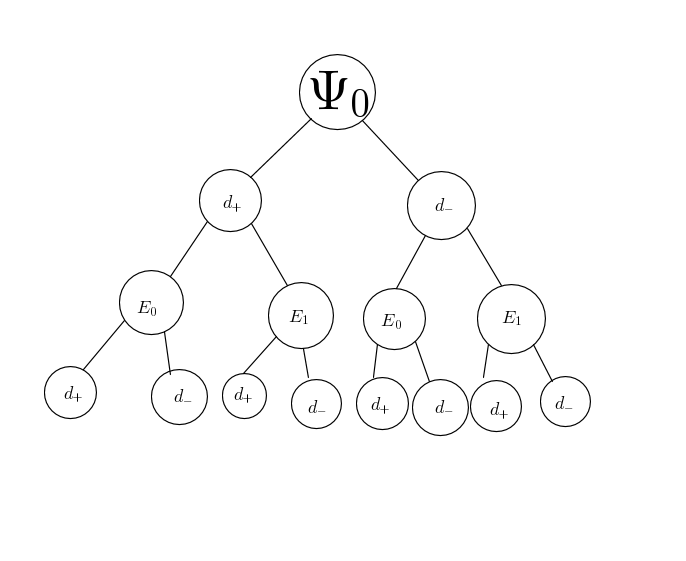
\includegraphics[scale=0.6]{3c.png}
\caption{Et valgtre som viser alle de mulige utfallene vi kan observere.}
\end{figure}

Vi stater med grunntilstanden $\Psi_0$, vi observerer deretter enten $d_+$ eller $d_-$. Bølgelikningen kollapser så til tilstanden som tilsvarer denne målingen ($|d_+\rangle$ eller $|d_-\rangle$). Vi observerer så energien, og måler enten $E_0$ eller $E_1$, og bølgefunksjonen kollapser til forholdsvis $|h_{10}\rangle$ eller $|h_{11}\rangle$. I den lange utregningen under bryter jeg min egen notasjon, og skriver $|E_0\rangle \equiv |h_{10}\rangle $ og $|E_1\rangle \equiv |h_{11}\rangle $, dette er for å gjøre det lettere å lese og skrive, så beklager om dette skaper forvirring, men nå er du advart! Vi gjør så en siste måling og får enten $d_+$ eller $d_-$.\\

Sannsynligheten for å gjøre en viss måling av en tilstand $| f_n\rangle$ når vi har en tilstand $|\psi_n\rangle$ er gitt ved:

$$
|c_n|^2 = |\langle f_n|\psi_n\rangle|^2
$$

(Vi har bare reelle tilstander, så vi kan fjerne $|$ $|$ for alle sannsynligheten, annet enn de for $\Psi(t)$)\\

Sannsynligheten for å måle samme $D$ begge gangene er

\begin{equation}
P(samme) = P(d_+ \cap d_+) + P(d_- \cap d_-)
\label{eq:Psamme}
\end{equation}

Vi finner så at leddene er gitt ved:

$$
P(d_+ \cap d_+) = P(d_+)P(d_+|d_+)
$$

$P(d_+|d_+)$ er sannsynligheten for at vi igjen måler $d_+$ etter vi har målt $d_+$ én gang. Dette er gitt ved sannsynligheten for at vi først måler $E_0$ så $d_+$ eller at vi måler $E_1$ så $d_+$. Så

$$
P(d_+|d_+) = \langle E_0|d_+\rangle^2\langle d_+|E_0\rangle^2 + \langle E_1|d_+\rangle^2\langle d_+|E_1\rangle^2
$$

$\langle E_0|d_+\rangle^2\langle d_+|E_0\rangle^2$ er sannsynligheten for at vi først måler $E_0$ så $d_+$, og $\langle E_1|d_+\rangle^2\langle d_+|E_1\rangle^2$ er sannsynligheten for at vi måler $E_1$ så $d_+$. 

$P(d_+)$ er gitt som:

$$
P(d_+) = |\langle d_+|\Psi\rangle|^2
$$

Vi får da:

$$
P(d_+ \cap d_+) = |\langle d_+|\Psi\rangle|^2\left[\langle E_0|d_+\rangle^2\langle d_+|E_0\rangle^2 + \langle E_1|d_+\rangle^2\langle d_+|E_1\rangle^2\right]
$$


Og helt tilsvarende:

$$
P(d_- \cap d_-) = |\langle d_-|\Psi\rangle|^2\left[\langle E_0|d_-\rangle^2\langle d_-|E_0\rangle^2 + \langle E_1|d_-\rangle^2\langle d_-|E_1\rangle^2\right]
$$

Vi ender da med at sannsynligheten er:

$$
P(samme) = |\langle d_+|\Psi\rangle|^2\left[\langle E_0|d_+\rangle^2\langle d_+|E_0\rangle^2 + \langle E_1|d_+\rangle^2\langle d_+|E_1\rangle^2\right] \\
$$
$$
+
 |\langle d_-|\Psi\rangle|^2\left[\langle E_0|d_-\rangle^2\langle d_-|E_0\rangle^2 + \langle E_1|d_-\rangle^2\langle d_-|E_1\rangle^2\right]
$$

Vi kan så begynne å regne ut dette beistet. Fra tidligere i oppgaven har vi funnet at:

$$
|E_0\rangle = 
\begin{pmatrix}
1\\0
\end{pmatrix}
, \qquad
|E_1\rangle = 
\begin{pmatrix}
0\\1
\end{pmatrix}
$$
$$
|d_+\rangle = 
\frac{1}{\sqrt{4-2\sqrt{2}}}
\begin{pmatrix}
-1+\sqrt{2}\\1
\end{pmatrix}
,\qquad
|d_+\rangle = 
\frac{1}{\sqrt{4+2\sqrt{2}}}
\begin{pmatrix}
-1-\sqrt{2}\\1
\end{pmatrix}
$$
$$
|\Psi(t)\rangle = \frac{1}{\sqrt{5}}
\begin{pmatrix}
2e^{-i(t_D-t_1)} \\ e^{-3i(t_D-t_1)}
\end{pmatrix}
$$

I uttrykket for $|\Psi(t)\rangle$ finner vi en stygg tidsavhengighet, som vi håper skal forsvinne. Vi kan så regne ut indreproduktene:

$$
\langle E_0|d_+\rangle^2 = \left(\frac{-1 + \sqrt{2}}{\sqrt{4-2\sqrt{2}}}\right)^2, \qquad \langle E_0|d_-\rangle^2 = \left(\frac{-1 - \sqrt{2}}{\sqrt{4+2\sqrt{2}}}\right)^2
$$
$$
\langle E_1|d_+\rangle^2 = \frac{1}{4-2\sqrt{2}} ,\qquad \langle E_1|d_-\rangle^2 = \frac{1}{4+2\sqrt{2}} 
$$

Indreprodukt er uavhenging av hvilke vei vi skriver dem, så

$$
\langle d_+|E_0\rangle^2 = \langle E_0|d_+\rangle^2 ,\qquad \langle d_-|E_0\rangle^2 = \langle E_0|d_-\rangle^2
$$
$$
\langle d_+|E_1\rangle^2 = \langle E_1|d_+\rangle^2 ,\qquad \langle d_-|E_1\rangle^2 = \langle E_1|d_-\rangle^2
$$

Vi regner ikke ut $\langle d_{\pm}|\Psi(t)\rangle$ enda, av grunner vi skal se senere! Vi kan nå regne ut leddene i sannsynligheten:

$$
P(d_+ \cap d_+) = |\langle d_+|\Psi\rangle|^2\left[\langle E_0|d_+\rangle^2\langle d_+|E_0\rangle^2 + \langle E_1|d_+\rangle^2\langle d_+|E_1\rangle^2\right]
$$
$$
= |\langle d_+|\Psi\rangle|^2\left[\langle E_0|d_+\rangle^2\langle E_0|d_+\rangle^2 + \langle E_1|d_+\rangle^2\langle E_1|d_+\rangle^2\right]
$$
$$
= |\langle d_+|\Psi\rangle|^2\left[\langle E_0|d_+\rangle^4 + \langle E_1|d_+\rangle^4\right]
$$
$$
= |\langle d_+|\Psi\rangle|^2\left[\left(\frac{-1+\sqrt{2}}{\sqrt{4-2\sqrt{2}}}\right)^4 + \left(\frac{-1-\sqrt{2}}{\sqrt{4+2\sqrt{2}}}\right)^4\right]
$$
$$
= \frac{3}{4}|\langle d_+|\Psi\rangle|^2
$$

Og tilsvarende:

$$
P(d_- \cap d_-) = |\langle d_-|\Psi\rangle|^2\left[\langle E_0|d_-\rangle^2\langle d_-|E_0\rangle^2 + \langle E_1|d_-\rangle^2\langle d_-|E_1\rangle^2\right]
$$
$$
= |\langle d_-|\Psi\rangle|^2\left[\langle E_0|d_-\rangle^4 + \langle E_1|d_-\rangle^4\right]
$$
$$
= |\langle d_-|\Psi\rangle|^2\left[ \left(\frac{1}{4-2\sqrt{2}}\right)^2 + \left(\frac{1}{4+2\sqrt{2}}\right)^2\right]
$$
$$
= \frac{3}{4}|\langle d_-|\Psi\rangle|^2
$$

Og her skjedde det noe utrolig vakkert! Sannsynligheten for at man ved første måling enten finner $d_+$ eller $d_-$ må være $1$. Dette vil si at $|\langle d_+|\Psi\rangle|^2 + |\langle d_-|\Psi\rangle|^2 = 1$. Så nå ser vi at:

\begin{equation}
P(samme) = P(d_+ \cap d_+) + P(d_- \cap d_-) = \frac{3}{4}\left(|\langle d_+|\Psi\rangle|^2 + |\langle d_-|\Psi\rangle|^2\right) = \underline{\underline{\frac{3}{4}}}
\end{equation}

Siden all tidsavhengighet lå i $\langle d_+|\Psi\rangle$ og $\langle d_-|\Psi\rangle$, og disse forsvant, så betyr det at tidsavhengigheten til sannsynligheten også ble borte, og det er til en hver tid like sannsynlig å måle samme måling to ganger på rad!\\


Så da har vi funnet at sannsynligheten for å måle samme verdi for $D$ ved to raske målinger er alltid $\underline{\underline{\frac{3}{4}}}$.

\subsection*{d)}

Fungerer maskinen skal vi kunne forvente å måte $\langle D\rangle$ gitt i \ref{eq:forventningD}. Men forventningsverdien til observablen $D$  er avhenging av energiene til $H_1$. Skrur maskinen seg av og systemet går over i regimet til $H_1$, så er tilstandene beskrevet av $|h_{00}\rangle$ og $|h_{01}\rangle$ og deres tilhørende energier $E_{00}$ og $E_{01}$. Dette betyr at forventningsverdien til $D$ ikke lenger er det samme.\\

Men hvordan kan vi faktisk sjekke dette? Merk at i \ref{eq:forventningD} hadde vi et $\cos(2(t_D - t_1)$-ledd. Dette leddet bestemmer hvordan forventningsverdien til $D$ varierer med tiden. Det er faktoren $2$ som bestemmer hvor fort disse verdiene varierer med tiden. Tar man nok målinger vil man kunne observere denne hastigheten. Denne hastigheten er, som nevnt over, bestemt av energiene til $H_1$, så når systemet går over i $H_0$ vil ikke denne hastigheten. Regner man litt på det kan man finne at forventningsverdien nå er avhengig av leddet $\cos(10(t_D - t_1)$. Så med andre ord oscillerer forventningsverdien 5 ganger raskere. Man kan derfor med nok målinger bestemme hvor raskt forventingsverdien oscillerer, og dermed finne om vi er i $H_1$ eller $H_0$, og derfor om maskinen har skrudd seg av.

\newpage

\section{Appendix:}
\subsection*{Kode for 1a)}

\lstinputlisting{solver.py}\label{lst:solver}

\end{document}


